%%&program=xelatex
%&encoding=UTF-8 Unicode
% SVN keywords
% $Author$
% $Date$
% $Revision$
% $URL$
\documentclass[a4paper,12pt]{article}  % Comments after  % are ignored
%\usepackage{hyperref}                 % For creating hyperlinks in cross references
%
\usepackage{ifxetex}% for XELATEX, or PDFlatex
\usepackage{ifplatform} 
%\usepackage{hyperref}
%\hypersetup{colorlinks=false}
%
\ifxetex
	\usepackage{polyglossia} \setmainlanguage{portuges}
	\usepackage{fontspec}
	\ifwindows
		\setmainfont[Ligatures=TeX]{Garamond}
		\setsansfont[Ligatures=TeX]{Gill Sans MT}
		\setmonofont{Consolas}
%		\setmonofont[Scale=MatchLowercase]{Courier}
	\fi
	\iflinux
		\setmainfont[Ligatures=TeX]{Linux Libertine O}
		\setsansfont[Ligatures=TeX,Scale=MatchLowercase]{Linux Biolinum}
		\setmonofont[Scale=MatchLowercase]{Courier}
	\fi
	\ifmacosx
	% add settings
	% Use xelatex -no-shell ...
	\fi
	\usepackage{xcolor,graphicx} 
\else
	\usepackage[portuguese]{babel}
	%\usepackage[latin1]{inputenc}
	\usepackage[utf8]{inputenc}
	\usepackage[T1]{fontenc}
	\usepackage{graphics}                 % Packages to allow inclusion of graphics
	\usepackage{color}                    % For creating coloured text and background
\fi

\usepackage{enumitem}
\setlist{nolistsep}

\usepackage{amsmath,amssymb,amsfonts} % Typical maths resource packages
\usepackage[retainorgcmds]{IEEEtrantools}
\usepackage{caption}

\usepackage{tikz}
\usetikzlibrary{calc,arrows,decorations.pathmorphing,intersections}
\usepackage[font={small,sf},labelfont={bf},labelsep=endash]{caption}
\usepackage{sansmath}

%use as the last command into the preamble 
\usepackage[bookmarks,colorlinks]{hyperref}

\oddsidemargin 0cm
\evensidemargin 0cm

\pagestyle{myheadings}         % Option to put page headers
                               % Needed \documentclass[a4paper,twoside]{article}
\markboth{{\small \it  Laboratório de Física Experimental Básica}}
{{\small\it MEFT - 1º Sem. 2014/2015} }

\addtolength{\hoffset}{-0.5cm}
\addtolength{\textwidth}{2.5cm}
\addtolength{\topmargin}{-1.5cm}
\addtolength{\textheight}{3cm}

%\textwidth 15.5cm
%\topmargin -1.5cm
\setlength{\parindent}{0pt}
\setlength{\parskip}{1ex  plus  0.5ex  minus  0.2ex}
%\parindent 0.5cm
%\textheight 25cm
%\parskip 1mm


% Math macros
\newcommand{\ud}{\,\mathrm{d}} 
\newcommand{\HRule}{\rule{\linewidth}{0.5mm}}

\author{Prof. Bernardo B. Carvalho} 

%%%%, Bernardo Brotas Carvalho\\bernardo.carvalho@tecnico.ulisboa.pt} 
\date{ Outubro 2014} 

\begin{document} 

	
\includegraphics[width=0.2\textwidth]{../logo-ist}%\\[1cm]  %%  Logo_IST_color

	\HRule \\[0.5cm]
	{ \huge \sf  \textsc{Efeito fotoeléctrico}} \\[0.4cm] % \bfseries 
%	{ \huge \sf  \textsc{Construções Geométricas em Lentes Delgadas (aproximação paraxial)} }\\[0.4cm] % \bfseries 
	{ \large \bfseries Determinação da constante de Planck.}\\
%	{ \large \bfseries Procedimento Experimental}\\
	\HRule \\%[0.5cm]

\section{\sf OBJECTIVO DO TRABALHO}
\begin{itemize}
\item Verificação experimental do efeito fotoeléctrico
\item Determinação da energia cinética dos fotoelectrões em função da frequência da luz incidente sobre a celula fotoeléctrica
\item  Determinação da constante de Planck, h
%\item  Verificação da não-dependência da energia cinética dos fotoelectrões na intensidade da luz incdente na celula fotoeléctrica.
\end{itemize}


\section{\sf INTRODUÇÃO }
%\section{\sf }
%\subsection{\sf }
%\subsection{\sf Corpo esférico em queda livre num fluido}
O efeito fotoelétrico era já conhecido no final do séc. XIX, com a emissão  de partículas carregadas da superfície de um metal quando ilumidas por luz intensa. No entanto  verificou-se que a energia destas partículas, que mais tarde foram indentificadas por eletrões, não dependia da intensidade mas sim do comprimento de onda da  luz incidente. A intensidade só determina o número de fotoeletrões emitidos. A explicação correcta do efeito fotoeléctrico foi proposta em 1905 por Einstein\footnote{Pela qual recebeu o prémio Nobel em 1921.} baseada na teoria de Max Planck\footnote{Teoria Quântica da luz, pela qual recebeu o prémio Nobel em 1918.} da emissão-absorção da luz. 

\begin{equation}
	\label{eq:energia2}
	E = h \nu = K_e^{max} + W_O
\end{equation}

Em que $K_e^{max}$ é a energia cinética máxima dos fotoeletrões  e $W_O$ é a energia necessária para remover os eletrões da superfície do material (\emph{Work function}, característica de cada metal). $E$ é então a energia do quantum de luz que se batizou como \emph{fotão}.

De acordo com esta teoria corpuscular da luz, quando um fotão incide sobre a superficie  de um sólido  é absorvido por um átomo, dá-se a libertação de um dos electrões de valência. A estes electrões tem de ser comunicada uma enegia 
 para que se libertem da rede metálica. Se o fotão incidente tiver mais energia que um limiar ($W_O$), o fotoelectrão sai do sólido com uma energia cinetica $K_e = h\nu - W_O$.
A figura \ref{fig:EFE}   representa esquematicamente o fotão incidente, a superfície do sólido, os níveis de energia dos electrões de valência do material. Note que se a energia do fotão incidente não for suficiente (se $E_f < W_O$) não há emissão de fotoelectrões.

 
\begin{figure}[htb]   
\begin{center}
  \sansmath
    \begin{tikzpicture}[scale=0.25]
    \begin{scope} % Energy levels
        \draw (1,0) node[left] {$1s$} -- 
            ++(14,0) node[right] {$K$};
        \draw (1,4) node[left] {$2s$} -- 
            ++(14,0) node[right] {$L_1$};
        \draw (1,6) node[left] {$2p$} -- 
            ++(14,0) node[right] {$L_2,L_3$};
        \draw (0,12) -- 
            ++(16,0) node[right] {Nível  de Fermi};
        \draw[line width=0.9mm, black!50!white] (0,18) -- 
            ++(20,0) node[right] {Superfície};
    \end{scope}
    \begin{scope} % Valence and conduction bands
%        \draw (-8,7) rectangle node {banda de valência} 
%            ++(14,4);
        \draw (-8,13) rectangle node {banda de condução} 
            ++(14,4);
    \end{scope}
    \begin{scope} % Electrons
        \foreach \x in {3,5,...,11}
            \filldraw (\x, 6) circle (.75);
        \draw (11, 6) circle (.75);
        \foreach \x in {7, 9}
            \filldraw (\x, 4) circle (.75);
        \foreach \x in {7, 9}
            \filldraw (\x, 0) circle (.75);
        %\filldraw (7,0) circle (.75);
        
        %\filldraw(9, 0) circle (.75);
        
    \end{scope} 
    \begin{scope}[color=blue] % X-rays in, electron out
        \draw[decorate, decoration=snake] (12,20) 
            node[above] {$h\nu_b$}  -- (7,5.75);
        \draw[->] (7,5.75) -- (1,20);
        \filldraw (0.4,22) circle (0.75) node[right=5] {fotoeletrão};
    \end{scope}
    \draw[color=green,decorate, decoration=snake] (15,20) 
     node[above] {$h\nu_g$}  -- (9,5.75);

    \begin{scope}[color=red] % X-rays in, electron out
        \draw[decorate, decoration=snake] (18,20) 
            node[above] {$h\nu_r$}
            -- (9,0.75);
        %\draw[->] (9,0.75) -- (1,20);
        %\filldraw (0.4,22) circle (0.75) node[right=5] {fotoeletrão};
    \end{scope}
        
    \end{tikzpicture}

	\caption{Efeito fotoeléctrico}
	 \label{fig:EFE} 
	\end{center}
\end{figure}
	  
%\section{\sf Princípio do método}

A constante de Planck pode ser determinada expondo a superficie de um metal a luz monocromática, caracterizada por um comprimento de onda $\lambda=c /\nu$, e medindo a energia cinética máxima dos fotoelectrões emitidos. A fig.~\ref{fig:plack_exp} representa esquematicamente uma montagem experimental para a realização desta experiência.

\begin{figure}[htb] 
	\centering 
	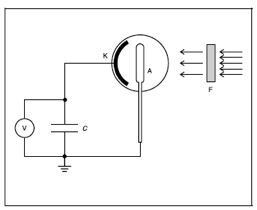
\includegraphics[width=0.6\textwidth]{planck_exp} 
	\caption{Diagrama esquematico da experiência do efeito fotoelétrico} \label{fig:plack_exp}
\end{figure}

%\begin{equation}
%	\label{eq:energia}
%	E= h \nu
%\end{equation}

A luz incide na superfície de metal, designado \emph{cátodo} (K), através de um \emph{ânodo} anelar ou transparente. 
Como cátodo é normalmente utilizado um metal alcalino (K, Na, Cd)  pois neste caso os electrões de valência estão fracamente 
ligados ao nucleo (i.e. têm uma função trabalho W baixa). Como ânodo utiliza-se por exemplo a platina  (Pt). 
O ânodo recebe parte dos fotoelectrões emitidos dando origem a uma corrente $I_f$. 
Se aplicarmos um potencial eléctrico retardador $V$ entre o ânodo e o cátodo a fotocorrente decresce, pois os fotoeletrões terão de vencer uma barreira de  potencial eletrostática $U=V e$, onde $e$ é a carga do electrão. 
Para uma dada tensão crítica $V_s$ (potencial de paragem), deixa de existir fotocorrente. Neste caso, mesmo os electrões mais fracamente ligados e que assim têm as maiores energias cinéticas, são parados. 
Experimentalmente pode-se usar uma fonte de tensão externa para aplicar o potencial de paragem ou mais simplesmente usa-se um condensador que carrega com a própria corrente dos fotoelectrões (Fig.~\ref{fig:plack_exp}) até esta ser eliminada. Neste caso é necessário utilizar um voltímetro de muito elevada impedância de entrada, ou um amplificador eletrónico de instrumentação, que é o caso da nossa experiência.

 Após medir o potencial de paragem, podemos assim escrever\footnote{Na realidade a função de trabalho tem de ser corrigida pelo potencial de contacto entre os dois metais, $W=W_O - \phi$, o que naturalmente não é importante para a determinação da constante de proporcionalidade.}:

%, onde $e$ é a carga do electrão) entre o ânodo e o cátodo,
\begin{equation}
	\label{eq:energia}
	e\,V_s= K_e^{max}= h \nu - W_O
\end{equation}

Medindo o potencial de paragem para varias frequências da luz incidente, podemos então fazer o gráfico de $V_s\; vs \;\nu$. Este gráfico é uma recta de declive $h/e$, e ordenada na origem  $-W/e$.


\begin{figure}[htb]   
\begin{center}
  \sansmath
    \begin{tikzpicture}[y=3cm, x=.01cm,font=\sffamily]
 	%axis
	\draw (0,0) -- coordinate (x axis mid) (800,0);
    \draw (0,0) -- coordinate (y axis mid) (0,1.7);
    	%ticks
    	\foreach \x in {0,100,...,800}
     		\draw (\x,1pt) -- (\x,-3pt)
			node[anchor=north] {\x};
    	\foreach \y in {0,0.5,1.,1.5}
     		\draw (1pt,\y) -- (-3pt,\y) 
     			node[anchor=east] {\y}; 
	%labels      
	\node[below=0.8cm] at (x axis mid) {$\nu$ [THz]};
	\node[rotate=90, above=0.8cm] at (y axis mid) {$V_s$ [V]};
	%linha
    \draw (360,0) -- (760,1.5) node[above] {$h/e$};
     %\filldraw (400,1) circle (0.75); %node[right=5] {fotoeletrão};
	 %Pontos
	 \draw plot[mark=*,only marks] file {hplot.data};

    \end{tikzpicture}

	\caption{Exemplo da determinação de $h$ pelo Efeito fotoeléctrico}
	 \label{fig:hplot} 
	\end{center}
\end{figure}

A constante $h$ é uma das constantes fisicas fundamentais que se conhece com maior precisão relativa ($u_r = 3.4\times 10^{-8}$). 
O valor actualmente reconhecido é de $h=6.62606889(23) \times 10^{-34}\,J\cdot s=4.135667516(91)\times 10^{-15}\,eV\cdot s$. 
(Os  dígitos em parentises representam a incerteza, tendo a mesma resolução dos dois últimos dígitos do valor). 
A contínua procura de um valor mais preciso não é apenas um puro desafio intelectual da comunidade científica.
 Terá um efeito prático revolucionário na Metrologia: 
 Como $h$ se pode relacionar com $N_A$, quando se conhecer com maior precisão\footnote{O dispositivo mais preciso é a balança de Watt, onde se espera chegar à precisão de $u_r \sim 1\times 10^{-11}$} será possível definir a unidade padrão de massa do sistema S.I. a partir da massa de um determinado átomo elemento químico, e portanto válido para todo o Universo. 
 O padrão de massa oficial é o último resistente do sistema MKS que é baseado num ``artefacto''; 
 um cilindro de platina-irídio guardado a \emph{sete chaves} em Sèvres nos subúrbios de Paris\footnote{Ver por exemplo o artigo da revista \href{http://www.economist.com/node/18007494}{Economist} http://www.economist.com/node/18007494}.   
 
\section{\sf Procedimento Experimental}

\begin{figure}[htb] 
	\centering 
	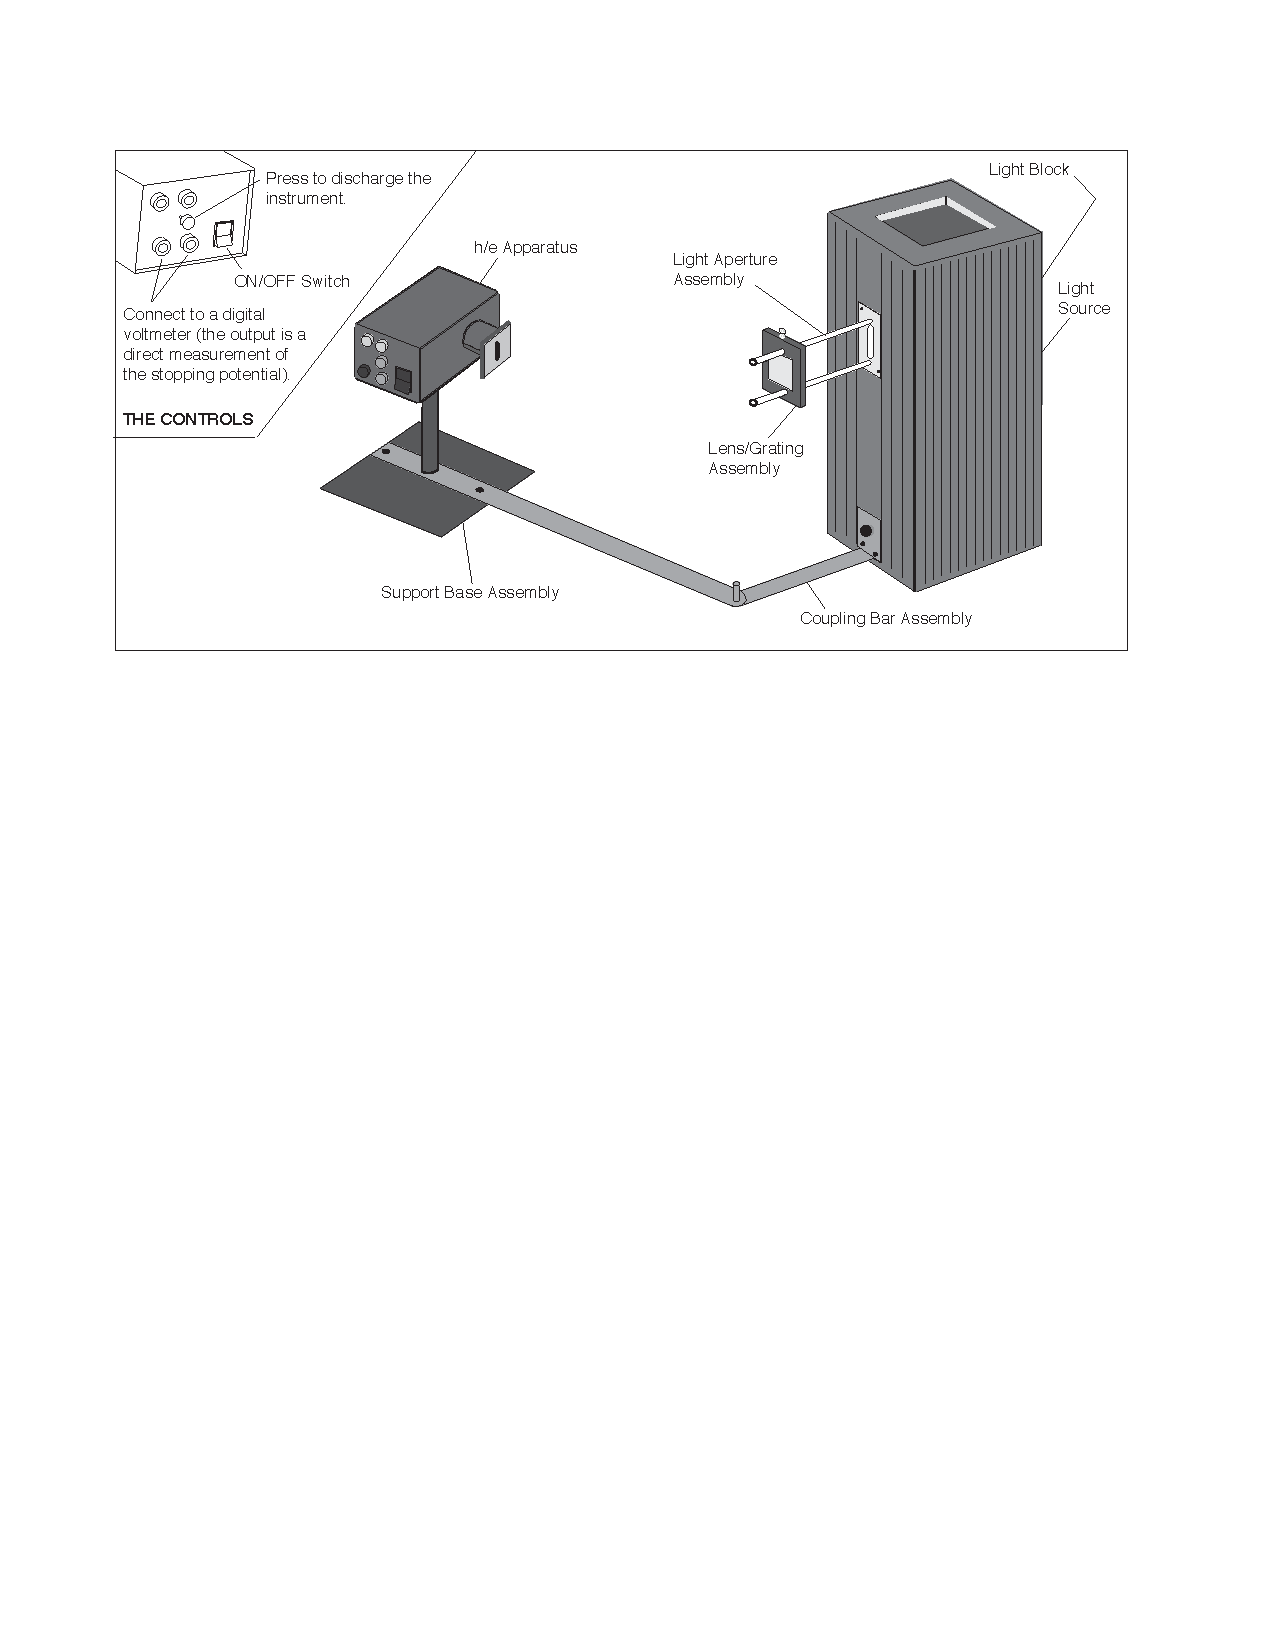
\includegraphics[width=0.8\textwidth]{planckPasco} 
	\caption{Montagem Experimental do efeito fotoelétrico} 
	\label{fig:plackPasco}
\end{figure}

\begin{enumerate}
\item Ligue a fonte de lâmpada de Mercúrio (Hg) e deixe estabilizar durante cerca de 10 min.
\item Enquanto espera, teste as tensõas das duas baterias do amplificador da célula fotovoltaica.
\item Monte os componentes tal como indicado na Fig.~\ref{fig:plackPasco}
\item Regule o conjunto de lente + rede de Difração de modo a obter as riscas de côr bem focadas na zona do detector. Alinhe a montagem para que a célula seja bem iluminada pelo feixe depois de passar pela fenda.
\item Observe as várias riscas, anote e interprete os ângulos de Difração e Ordem. A figura é simétrica  no que toca às posições e  intensidades observadas?
\item Para cada uma das riscas, depois de pressionar o botão de RESET, anote o valor da tensão de paragem e o tempo aproximado até esta estabilizar.
\item Repita o ponto anterior para outras duas riscas (côres) e com pelo menos dois filtros de transmissão.
\end{enumerate}


\begin{table}[!hbp]
\begin{center}
	%\centering
	\begin{tabular}{|c|c|c|}
	\hline
	Côr  & Freq [THz] & $\lambda$ [nm]  \\
	\hline
	Amarelo & 518.672 & 578 \\
	Verde & 548.996 & 546.074\\
	Azul & 687.858  & 435.835 \\
	Violeta & 740.858  & 404.656\\
	U.V.    & 820.264  & 365.483 \\
	\hline
 	\end{tabular}
	\caption{Riscas observáveis do espectro de Mercúrio} 
	\label{tab:Hg}
	\end{center}
\end{table}

Pode consultar o espectro de Mercúrio em  \href{http://physics.nist.gov/asd}{
NIST Atomic Spectra Database}, esconhendo o elemento ``Hg I" e um \emph{Relative intensity minimum:} de $1000$, por exemplo. 	  	



%\newpage
%\section*{\sf Apêndice}



\end{document} 